% VSMT-lean manuscript, S4 draft (RA-L format, ruling 113-4). Claims follow docs/METHOD.md section 2
% ("claim scope after S3-05", ruling 113) and the sentence-level wording of EXECUTE LOG-307 A2/A4, LOG-308 and LOG-309.
% Tables are generated by paper/tools/make_tables.py and data figures by paper/tools/make_figures.py from committed
% results/; do not edit paper/tables/*.tex or paper/figures/*.pdf by hand.
\documentclass[letterpaper,journal,twoside]{IEEEtran}

% ---------------------------------------------------------------------------------------------------------------
% Version switch (the only place). Review version (default): anonymous for RA-L double-blind review -- the author
% slot is kept but carries no author information, and every release link is withheld. Final version: authors and
% links. On Overleaf change \finalversionfalse to \finalversiontrue; paper/tools/build.sh builds both versions at
% once (build/vsmt_review.pdf, build/vsmt_final.pdf) by defining \VSMTFINAL for the final one.
\newif\iffinalversion
\finalversionfalse
\ifdefined\VSMTFINAL \finalversiontrue \fi
% the anonymous version also leaves the creation date (with its time zone) and the trailer ID out of the PDF
\iffinalversion\else\ifdefined\pdfinfoomitdate \pdfinfoomitdate=1 \pdftrailerid{}\fi\fi
% ---------------------------------------------------------------------------------------------------------------

\usepackage{amsmath,amssymb}
\usepackage{booktabs}
\usepackage{graphicx}
\usepackage{tikz}
\usetikzlibrary{positioning,arrows.meta,calc}
\usepackage{xcolor}
\usepackage{pifont} % check and cross marks in Fig. 1
\usepackage{url}
\makeatletter\g@addto@macro\UrlBreaks{\do\_}\makeatother % long file names may break at underscores
\usepackage[hidelinks]{hyperref}
\usepackage{cite}

% Draft markers: every [TODO]/[VERIFY] must be resolved before submission.
\newcommand{\todo}[1]{\textcolor{red}{[TODO: #1]}}
\newcommand{\verifyref}[1]{\textcolor{orange}{[VERIFY: #1]}}
\newcommand{\arm}[1]{\textsc{#1}}
\newcommand{\op}[1]{\texttt{#1}}
% Release locations: printed only in the final version.
\newcommand{\withheld}{(link withheld for review)}
\newcommand{\coderepo}{\iffinalversion\url{https://github.com/JingzeSun/VSMT}\else\withheld\fi}

\begin{document}
\bstctlcite{IEEEexample:BSTcontrol}

\title{Versioned Lifecycle Transactions for Object-Level Spatial Memory:\\ A Pre-Registered Evaluation Under Unobserved Changes}

\iffinalversion
\author{Jingze Sun%
\thanks{Manuscript draft, \today.}%
\thanks{J.~Sun is with The University of Sydney, Sydney, NSW 2006, Australia (e-mail: jingzesun498@gmail.com).}}
\markboth{IEEE Robotics and Automation Letters. Preprint Version. Draft}{Sun: Versioned Lifecycle Transactions for Object-Level Spatial Memory}
\else
\author{Anonymous Authors%
\thanks{Manuscript draft, \today.}%
\thanks{Author names, affiliations and contact details are withheld for double-blind review.}}
\markboth{IEEE Robotics and Automation Letters. Preprint Version. Draft}{Anonymous: Versioned Lifecycle Transactions for Object-Level Spatial Memory}
\fi

\maketitle

% Abstract. Ruling 113 requires three statements here: SAM 2.1 identity continuity does not improve; with instance masks
% ELU-P has the lower Missing residual rate, together with its false retractions; node F1 is reported as a difference only.
% Ruling 113-1 also requires, next to the instance-mask claim: near-ideal segmentation, and that the inference target is
% the training procedure (five seeds). Forbidden in title and abstract: robust, across segmenters, outperform(s), state of the art.
\begin{abstract}
A robot revisiting a changed home must decide, for each remembered object it cannot confirm, whether it is occluded, missed, removed or moved, and must restore a moved object's identity when it reappears.
We study VSMT-lean, an object-level memory updated by versioned transactions over five atoms (keep, bind, birth, retract, reactivate); a retraction closes a version instead of deleting it, so a later reactivation can restore the identity.
Small cost heads over a frozen RGB-D front end learn from hindsight instance-truth labels, which are read only after candidates and features are sealed.
The primary hypothesis, testing order and analysis plan were frozen before validation or test data were read; the test ran once on ProcTHOR houses (87 with instance masks, 85 with SAM~2.1 masks).
With simulator instance masks, which segment almost perfectly, the training procedure (five seeds) leaves fewer stale entities and keeps more identities than the same-recipe association-only ablation: the Missing residual rate falls from 0.642 to 0.115 and identity continuity rises from 0.104 to 0.211 (two-level one-sided 95\% lower bounds 0.467 and 0.049).
With SAM~2.1 masks stale entities also fall (0.235 to 0.055), but identity continuity does not improve (0.063 vs.\ 0.082).
Node F1 differs from the ablation by $+0.003$ and $+0.009$; no non-inferiority margin was registered.
No method leads on every metric: with instance masks a rule-based persistence filter leaves fewer stale entities (0.075 vs.\ 0.115), while 92.4\% of the in-scope entities it retracts belong to objects still in place.
In a descriptive ablation, deleting instead of retracting leaves slightly fewer stale entities but drops identity continuity to near zero.
\end{abstract}

\begin{IEEEkeywords}
Mapping, semantic scene understanding, object-level memory, long-term autonomy.
\end{IEEEkeywords}

\section{Introduction}
\label{sec:intro}

\begin{figure}[t]
\centering
% Fig. 1 (page-1 overview), TikZ; included by sections/introduction.tex. Drawn by hand from docs/METHOD.md sections 3-4
% and 11 (metric definitions); no data. A cup is moved from the table to the shelf while unseen: what a memory that only
% binds and births (AssocOnly), one that deletes (NoVersion) and VSMT-lean can do, and what the two primary metrics score.
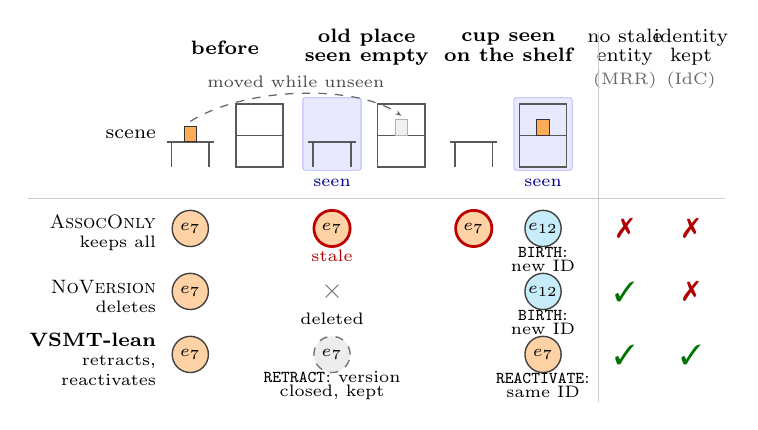
\begin{tikzpicture}[x=1mm, y=1mm, font=\scriptsize,
  furn/.style={draw=black!65, line width=0.55pt},
  cup/.style={draw=black!80, fill=orange!65, line width=0.3pt},
  faded/.style={draw=black!30, fill=black!6, line width=0.3pt},
  seen/.style={fill=blue!9, draw=blue!30, line width=0.3pt, rounded corners=0.8pt},
  ent/.style={circle, draw=black!75, line width=0.5pt, inner sep=0pt, minimum size=4.6mm, font=\fontsize{6}{6.6}\selectfont},
  same/.style={ent, fill=orange!35},
  newid/.style={ent, fill=cyan!22},
  stale/.style={ent, fill=orange!35, draw=red!75!black, line width=1pt},
  closed/.style={ent, fill=black!7, draw=black!55, dashed},
  note/.style={font=\fontsize{6}{6.6}\selectfont, align=center, inner sep=0.4pt},
  head/.style={font=\scriptsize\bfseries, align=center, inner sep=0.5pt},
  outhead/.style={font=\scriptsize, align=center, inner sep=0.5pt},
  row/.style={font=\scriptsize, align=right, anchor=east, inner sep=0.5pt},
  good/.style={text=green!45!black, font=\normalsize},
  bad/.style={text=red!70!black, font=\normalsize},
]
% column centres: three moments, then the two outcomes
\def\Xa{24}\def\Xb{42}\def\Xc{60}\def\Oa{74.8}\def\Ob{83.2}
% ---- headers
\node[head] at (\Xa, 3) {before};
\node[head] at (\Xb, 3) {old place\\[-1pt]seen empty};
\node[head] at (\Xc, 3) {cup seen\\[-1pt]on the shelf};
\node[outhead] at (\Oa, 3) {no stale\\[-1pt]entity};
\node[outhead] at (\Ob, 3) {identity\\[-1pt]kept};
\node[note, text=black!60] at (\Oa, -1.2) {(MRR)};
\node[note, text=black!60] at (\Ob, -1.2) {(IdC)};
% ---- scene row: a table (left) and a shelf (right) at each moment
\node[row] at (15.5, -8) {scene};
\fill[seen] (\Xb-8.1, -12.6) rectangle (\Xb-0.7, -3.4);
\fill[seen] (\Xc+0.7, -12.6) rectangle (\Xc+8.1, -3.4);
\foreach \X in {\Xa, \Xb, \Xc} {
  \draw[furn] (\X-7.4, -9) -- (\X-1.4, -9);
  \draw[furn] (\X-6.8, -9) -- (\X-6.8, -12.2) (\X-2, -9) -- (\X-2, -12.2);
  \draw[furn] (\X+1.4, -12.2) rectangle (\X+7.4, -4.2);
  \draw[furn] (\X+1.4, -8.2) -- (\X+7.4, -8.2);
}
\draw[cup] (\Xa-5.2, -9) rectangle (\Xa-3.6, -7.0);
\draw[faded] (\Xb+3.6, -8.2) rectangle (\Xb+5.2, -6.2);
\draw[cup] (\Xc+3.6, -8.2) rectangle (\Xc+5.2, -6.2);
\draw[->, >={Stealth[length=2.2pt]}, dashed, black!60, line width=0.45pt]
  (\Xa-4.4, -6.4) .. controls (\Xa+3, -1.8) and (\Xb-1, -1.8) .. (\Xb+4.4, -5.7);
\node[note, text=black!70, fill=white] at ({(\Xa+\Xb)/2}, -1.4) {moved while unseen};
\node[note, text=blue!55!black] at (\Xb-4.4, -14.2) {seen};
\node[note, text=blue!55!black] at (\Xc+4.4, -14.2) {seen};
\draw[black!20, line width=0.3pt] (-1, -16.2) -- (87.5, -16.2);
% ---- memory rows
\node[row] at (15.5, -20.6) {\arm{AssocOnly}\\[-1pt]\fontsize{6}{6.6}\selectfont keeps all};
\node[row] at (15.5, -28.6) {\arm{NoVersion}\\[-1pt]\fontsize{6}{6.6}\selectfont deletes};
\node[row] at (15.5, -36.6) {\textbf{VSMT-lean}\\[-1pt]\fontsize{6}{6.6}\selectfont retracts,\\[-1pt]\fontsize{6}{6.6}\selectfont reactivates};
% AssocOnly: the old entity stays (stale), the cup on the shelf gets a new identity
\node[same] at (\Xa-4.4, -20) {$e_7$};
\node[stale] at (\Xb-4.4, -20) {$e_7$};
\node[note, text=red!70!black] at (\Xb-4.4, -23.5) {stale};
\node[stale] at (\Xc-4.4, -20) {$e_7$};
\node[newid] at (\Xc+4.4, -20) {$e_{12}$};
\node[note] at (\Xc+4.4, -23.9) {\op{BIRTH}:\\[-1.5pt]new ID};
% NoVersion: retraction deletes the entity, so the cup can only be born again
\node[same] at (\Xa-4.4, -28) {$e_7$};
\node[note, font=\normalsize, text=black!55] at (\Xb-4.4, -28) {$\times$};
\node[note] at (\Xb-4.4, -31.5) {deleted};
\node[newid] at (\Xc+4.4, -28) {$e_{12}$};
\node[note] at (\Xc+4.4, -31.9) {\op{BIRTH}:\\[-1.5pt]new ID};
% VSMT-lean: retraction closes a version, reactivation reopens the same identity at the new place
\node[same] at (\Xa-4.4, -36) {$e_7$};
\node[closed] at (\Xb-4.4, -36) {$e_7$};
\node[note] at (\Xb-4.4, -39.9) {\op{RETRACT}: version\\[-1.5pt]closed, kept};
\node[same] at (\Xc+4.4, -36) {$e_7$};
\node[note] at (\Xc+4.4, -39.9) {\op{REACTIVATE}:\\[-1.5pt]same ID};
% ---- outcomes (check: good, cross: bad)
\node[bad] at (\Oa, -20) {\ding{55}}; \node[bad] at (\Ob, -20) {\ding{55}};
\node[good] at (\Oa, -28) {\ding{51}}; \node[bad] at (\Ob, -28) {\ding{55}};
\node[good] at (\Oa, -36) {\ding{51}}; \node[good] at (\Ob, -36) {\ding{51}};
\draw[black!20, line width=0.3pt] (71.4, 5) -- (71.4, -42);
\end{tikzpicture}

\caption{The problem on one cup, moved from the table to the shelf while the robot is away. Circles are \emph{entities}, the memory's records of believed objects. A memory that can only bind and birth (\arm{AssocOnly}) typically keeps a stale entity and gives the cup a new identity (it keeps the identity only by binding the cup's new fragment to its old, still active entity); one that deletes (\arm{NoVersion}) loses the identity; VSMT-lean retracts the entity, closing its version without deleting it, and can reactivate it on the shelf. The Missing residual rate (MRR) counts removed or moved objects with an entity left at their old place after it was seen empty; identity continuity (IdC) counts moved objects whose first new observation is attached to the entity that carried them before. Illustration, not data.}
\label{fig:overview}
\end{figure}

\IEEEPARstart{O}{bject-level} maps let a robot answer where things are without re-exploring~\cite{fusionpp2018,conceptgraphs2024,hydra2022}.
In a home, objects are taken away, moved and added while the robot is elsewhere, and every remembered object it then fails to see poses the same question: is it hidden, missed by the detector, removed, or moved (Fig.~\ref{fig:overview})?
A memory that keeps everything leaves \emph{stale entities}, records of objects at places they have left, which the Missing residual rate of the Dyn-THOR benchmark measures~\cite{dsg2026}; one that deletes aggressively removes objects that were only hidden, and a deleted object comes back under a new identity when it reappears elsewhere.
Most systems decide these cases with hand-set rules: threshold fusion~\cite{conceptgraphs2024}, existence probabilities or persistence filters~\cite{fusionpp2018,rosen2016persistence,perpetua2025}, or rendering the map and comparing it with the current view~\cite{dsg2026,dynamicgsg2025}.
We ask a narrower question than ``which system is best'': does a \emph{learned, reversible} lifecycle vocabulary reduce stale entities and keep identities, compared with the same learned association without that vocabulary, when everything else is held fixed?

We study VSMT-lean, the entity-lifecycle core of versioned structural memory transactions (the full design also revises places and relations, which we leave out).
The input is a stream of RGB-D frames with the simulator's camera poses, so there is no localization error; a frozen perception front end turns each frame into anonymous mask \emph{fragments}, image segments with geometry and an appearance descriptor but no object identity.
Every frame, one joint assignment decides for every fragment whether it is new evidence for an existing entity (\op{BIND}), a returning entity (\op{REACTIVATE}) or a new object (\op{BIRTH}); an existence head decides, for every entity that should be visible but was not matched, whether to keep it (\op{NOOP}) or \op{RETRACT} it.
A retracted entity leaves the map, but its closed version is kept, so the same identity can be reactivated later.
In the memory, only three small cost heads (54,787 parameters) are learned, from \emph{hindsight} labels: after the decision, the simulator's instance ground truth at that frame states which choice would have been right; these labels serve training and error analysis and are never an input.

The test rests on one counterfactual, \arm{AssocOnly}: the same association head and solver, retrained with the same recipe, with only \op{BIND} and \op{BIRTH}; without an existence step it never retracts, reactivates or marks an entity dormant.
It removes the learned lifecycle as a whole, not the learning, whose role \arm{HandCost} probes.
The primary hypothesis (a lower Missing residual rate, MRR, and a higher identity continuity, IdC, than \arm{AssocOnly}; Fig.~\ref{fig:overview}), its testing order over two front ends (simulator instance masks, then the learned segmenter SAM~2.1~\cite{sam2_2025}) and the statistics were frozen in versioned configuration files before validation or test data were read, and the test was run once.
We call this pre-registration; it is internal to the project, the hypothesis was revised after development and confirmation readings, and Section~\ref{sec:stats} discloses that history.
All nine compared methods (\emph{arms}, Table~\ref{tab:arms}) read byte-identical front-end outputs and share recall, deduplication, executor and evaluator.
Our contributions are:
\begin{enumerate}
\item A versioned, reversible lifecycle revision with learned costs, tested against an association-only counterfactual trained with the same recipe: with near-ideal instance masks the training procedure (five seeds) leaves fewer stale entities and re-attaches more relocated objects; with SAM~2.1 masks only the first part holds. A descriptive deletion ablation indicates that, on ProcTHOR, re-attachment depends on keeping the versions of retracted entities.
\item An auditable training and evaluation protocol: candidates sealed before labels are read, a ledger assigning every decision to exactly one class that separates three sources of error, and a pre-registered test with a single test read.
\item A same-front-end, metric-by-metric comparison with re-implemented association, persistence and render-and-compare mechanisms on two front ends, with a descriptive check on real rescans~\cite{rio2019}.
\end{enumerate}

\section{Related Work}
\label{sec:related}

\textbf{Object-level and scene-graph maps.}
Fusion++ maintains object-level TSDF volumes with an existence probability per object~\cite{fusionpp2018}.
3D scene graphs organise objects, places and rooms in layers~\cite{dsg3d2020,hydra2022}, and open-vocabulary systems such as ConceptGraphs associate 2D masks into 3D objects by thresholded geometric and semantic similarity~\cite{conceptgraphs2024}.
These systems mainly target static scenes; apart from existence probabilities as in Fusion++, a stale object is usually fused with new evidence or kept.

\textbf{Change-aware and long-term mapping.}
Persistence filters model the survival time of features in semi-static environments~\cite{rosen2016persistence}, and Perpetua extends this to emergence and persistence of objects~\cite{perpetua2025}.
Volumetric approaches detect object-level changes and update submaps~\cite{pocd2022,panopticmultitsdf2022}, and Khronos estimates the spatio-temporal history of a scene~\cite{khronos2024}.
Closest to our setting, DSG builds dynamic scene graphs in changing indoor environments with render-and-compare removal and introduces Dyn-THOR, with node precision, recall and F1 at 3D IoU 0.3 and the Missing residual rate~\cite{dsg2026}; DynamicGSG updates a Gaussian scene graph by rendering~\cite{dynamicgsg2025}.
DSG and DynamicGSG update with hand-set rules, and their removal takes the object out of the map; persistence models~\cite{rosen2016persistence,perpetua2025} and spatio-temporal maps~\cite{khronos2024} keep information about objects that disappear and re-emerge, through probabilistic models or optimisation rather than costs learned from labels.
We keep the metric definitions of Dyn-THOR where possible, implement their core mechanisms as adapters on our shared front end (Section~\ref{sec:arms}), and ask a different question: whether learned, reversible lifecycle operations add value over learned association alone.
Our adapters are independent implementations of published mechanisms, not reproductions of these systems.

\textbf{Learned memory operations.}
LLM memory systems choose operations such as add, update and delete with a frozen language model~\cite{mem0_2025}; we report a zero-training LLM operator on the same sealed feature tables only in the appendix.
Training on the model's own memory trajectories follows the data-aggregation idea of DAgger~\cite{dagger2011}.
As in work that pairs frozen pre-trained features with a small learned module~\cite{dinowm2025}, the front end (DINOv2 descriptors~\cite{dinov2_2024}, depth geometry and masks) is frozen, so differences between arms come from the memory logic alone.

\section{Method}
\label{sec:method}

\begin{figure*}[t]
\centering
\resizebox{\textwidth}{!}{% Fig. 2 (one frame of VSMT-lean), TikZ; included by sections/method.tex. Drawn by hand from docs/METHOD.md sections
% 3-8; no data. Frozen front end -> recall and sealed features -> joint assignment -> existence decisions -> executor;
% the teacher (training only) labels the sealed rows and columns; bottom right: the entity states (the map is the set
% of active and dormant entities; a retracted entity is out of the map but stays recallable). The cup example of
% Fig. 1 is not repeated here.
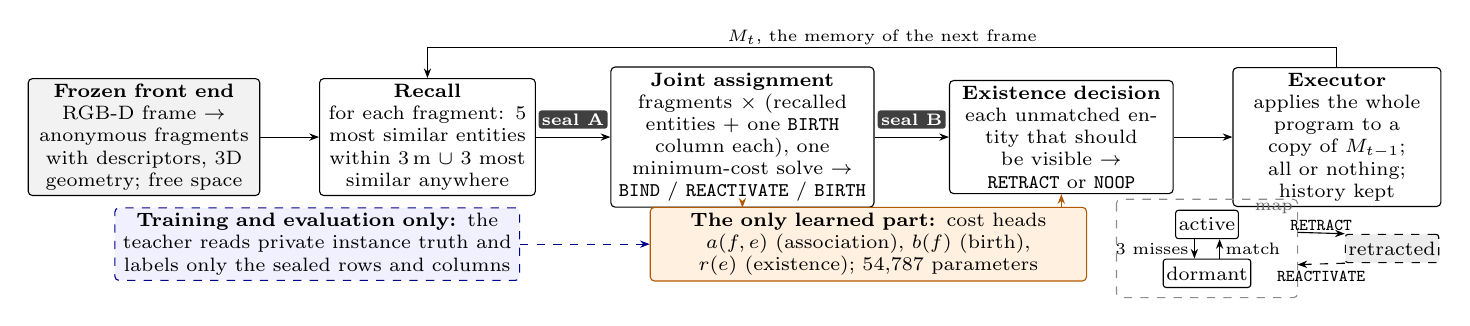
\begin{tikzpicture}[
  font=\scriptsize, >={Stealth[length=3.5pt]},
  box/.style={draw, rounded corners=1.5pt, align=center, inner sep=2pt, fill=white, minimum height=12mm},
  learned/.style={draw=orange!70!black, fill=orange!12, rounded corners=1.5pt, align=center, inner sep=2pt, minimum height=6mm},
  private/.style={draw=blue!55!black, fill=blue!6, dashed, rounded corners=1.5pt, align=center, inner sep=2pt, minimum height=6mm},
  seal/.style={fill=black!75, text=white, rounded corners=1pt, inner sep=1.2pt, font=\fontsize{6}{6.6}\selectfont\bfseries},
  lab/.style={font=\fontsize{6}{6.6}\selectfont, align=center, inner sep=0.8pt},
  st/.style={draw, rounded corners=1pt, font=\scriptsize, inner sep=1.1pt, minimum height=3.6mm, fill=white},
]
\node[box, fill=gray!10, text width=28mm] (fe) at (15mm, 0)
  {\textbf{Frozen front end}\\RGB-D frame $\to$ anonymous fragments with descriptors, 3D geometry; free space};
\node[box, text width=26mm] (rec) at (51mm, 0)
  {\textbf{Recall}\\for each fragment: 5 most similar entities within 3\,m $\cup$ 3 most similar anywhere};
\node[box, text width=32mm] (asg) at (91mm, 0)
  {\textbf{Joint assignment}\\fragments $\times$ (recalled entities + one \op{BIRTH} column each), one minimum-cost solve $\to$ \op{BIND} / \op{REACTIVATE} / \op{BIRTH}};
\node[box, text width=27mm] (ex) at (131.5mm, 0)
  {\textbf{Existence decision}\\each unmatched entity that should be visible $\to$ \op{RETRACT} or \op{NOOP}};
\node[box, text width=25mm] (exe) at (166.5mm, 0)
  {\textbf{Executor}\\applies the whole program to a copy of $M_{t-1}$; all or nothing; history kept};
\draw[->] (fe) -- (rec);
\draw[->] (rec) -- node[seal, above=1mm] {seal A} (asg);
\draw[->] (asg) -- node[seal, above=1mm] {seal B} (ex);
\draw[->] (ex) -- (exe);
\draw[->] (exe.north) -- ++(0, 2.5mm) -| node[lab, pos=0.25, above] {$M_t$, the memory of the next frame} (rec.north);
\node[learned, text width=54mm] (heads) at (107mm, -13.6mm)
  {\textbf{The only learned part:} cost heads $a(f,e)$ (association), $b(f)$ (birth), $r(e)$ (existence); 54,787 parameters};
\draw[->, orange!70!black] (heads.north -| asg) -- (asg.south);
\draw[->, orange!70!black] (heads.north -| ex) -- (ex.south);
\node[private, text width=50mm] (teach) at (37mm, -13.6mm)
  {\textbf{Training and evaluation only:} the teacher reads private instance truth and labels only the sealed rows and columns};
\draw[->, dashed, blue!55!black] (teach) -- (heads);
% entity states
\draw[black!45, dashed, rounded corners=1.5pt] (138.5mm, -7.9mm) rectangle (161.5mm, -20.4mm);
\node[font=\fontsize{6}{6.6}\selectfont, text=black!60, anchor=north east, inner sep=0.6pt] at (161.2mm, -8.2mm) {map};
\node[st] (sA) at (150mm, -11.1mm) {active};
\node[st] (sD) at (150mm, -17.3mm) {dormant};
\draw[->] ([xshift=-1.6mm]sA.south) -- node[lab, left=0.4mm] {3 misses} ([xshift=-1.6mm]sD.north);
\draw[->] ([xshift=1.6mm]sD.north) -- node[lab, right=0.4mm] {match} ([xshift=1.6mm]sA.south);
\node[st, fill=black!7, dashed] (sR) at (173.5mm, -14.15mm) {retracted};
\draw[->] (161.5mm, -12.1mm) -- node[lab, above] {\op{RETRACT}} (sR.north west);
\draw[->, dashed] (sR.south west) -- node[lab, below=0.6mm] {\op{REACTIVATE}} (161.5mm, -16.2mm);
\end{tikzpicture}
}
\caption{(a) One frame. Recall sets and association and birth features are sealed before any private file is opened (A), assignments and existence features after the solve (B); the teacher labels only sealed rows and columns, in training only. Orange: the only learned part. (b) A cup moved out of view: VSMT-lean reactivates the same identity, \arm{NoVersion} and \arm{AssocOnly} create a new one, and \arm{AssocOnly} also keeps a stale entity. Illustration, not data.}
\label{fig:method}
\end{figure*}

\subsection{Problem, memory and the five atoms}
Fig.~\ref{fig:method} summarises one frame and the lifecycle of a moved object.
At frame $t$ the memory receives public observations $O_t$ from a frozen front end---anonymous mask fragments with descriptors and 3D geometry, free-space and visibility evidence from depth, and the causal pose---and its own previous memory $M_{t-1}$; it outputs a frame program $\Pi_t$ and $M_t=\mathrm{exec}(M_{t-1},\Pi_t)$.
No simulator object identity, ground-truth mask, intervention log or future observation is an input; the executor is fixed, and what is learned is how $\Pi_t$ is chosen.
The memory is a set of entity records holding an anonymous identity, a state in $\{\text{active},\text{dormant},\text{retracted}\}$, a version chain (predecessor, opening and closing frame, closing transaction), a running-mean and a best-view descriptor, the centroid and box of the surface seen in the most recent frame, observation and missed-opportunity counts, and the evidence list.
\op{NOOP} keeps an unmatched, should-be-visible entity and increments its missed-opportunity count; \op{BIND} attaches a fragment to an active entity; \op{BIRTH} creates an entity from an unassigned fragment; \op{RETRACT} closes the current version of an unmatched, should-be-visible entity whose existence head fires, keeping its evidence and history; \op{REACTIVATE} opens a new version of a dormant or retracted entity at the new place, with the same identity.
A replacement is the composite \op{RETRACT}+\op{BIRTH}.
A shared rule moves an active entity to dormant (``not seen for a while, no evidence of absence'') after three consecutive missed opportunities and back on any match (\arm{AssocOnly} has no dormant state); retracted means ``evidence that it is no longer there''.
A shared deduplication runs every 10 frames over active and dormant entities (cosine $\geq 0.6$, centroid distance $\leq 0.5$\,m, box IoU $\geq 0.05$) and folds one record into the other, keeping all evidence.
The executor applies the whole program on a clone of $M_{t-1}$, checks every precondition and rolls the frame back if any atom fails; history is never physically deleted.

\subsection{Frozen front end}
Fragments come from the simulator's per-frame instance segmentation, of which only anonymous boolean masks are exposed, or from SAM~2.1 (Hiera Small, automatic mask generation)~\cite{sam2_2025,sam21release}; each covers at least 196 pixels, at most 64 per frame.
A fragment carries the mean DINOv2 ViT-B/14 patch token in its mask~\cite{dinov2_2024}, passed through a frozen 128-dimensional projection trained once per mask source on 30 development houses disjoint from all training, selection and test houses, and its back-projected points, centroid and box.
Whether an entity should be visible, and how much of its last seen surface is now seen through, is computed per arm from the public depth and $M_{t-1}$ by a shared function.
Instance masks remove segmentation error unrelated to memory but expose no identity; SAM~2.1 masks test whether conclusions hold with a learned segmenter.

\subsection{Recall and frame-level joint assignment}
For each fragment $f$, recall unites a local channel (top $k{=}5$ entities by cosine within 3\,m) and a global channel (top $k'{=}3$, any distance, any state); eligibility does not depend on the entity state, so \arm{AssocOnly} receives the same far-away candidates as VSMT-lean.
The cost matrix has a row per fragment and a column per recalled entity plus one \op{BIRTH} column per fragment,
\begin{equation}
C[f,e]=-a(f,e),\qquad C[f,\mathrm{birth}_f]=-b(f),
\label{eq:cost}
\end{equation}
with association and birth logits $a$, $b$ and a forbidding cost for unrecalled pairs.
A minimum-cost rectangular assignment~\cite{kuhn1955}, canonicalised to the lexicographically smallest optimum, is compiled into \op{BIND} (active entity), \op{REACTIVATE} (dormant or retracted entity) or \op{BIRTH}: it decides in one step who is whom, who is new and who is back, and the learned heads only supply the costs.
For every unassigned, should-be-visible active or dormant entity, the existence head then decides \op{RETRACT} or \op{NOOP}.

\subsection{Learned cost heads}
The association head $a(f,e)$ reads 14 features (descriptor cosines, centroid distance, box IoU, size ratio, time since last seen, missed opportunities, state, cosine rank and margin, mutual best match, support-height difference); the existence head $r(e)$ reads 17 (visible fraction, free-space coverage of the last seen surface, viewing distance and angle, counts, time since last seen, best cosine to a current fragment and whether it is unassigned, state, and five history counters of see-through runs at coverage $\geq 0.70$ and $\geq 0.85$, matches since birth, judgeable frames and accumulated coverage); the birth head $b(f)$ reads 4.
Each head standardises its fields with training-house statistics (counts log-transformed) and applies a two-layer, 128-wide GELU MLP: 54,787 parameters in all (\arm{AssocOnly}: 35,842).
The loss is a softmax cross-entropy over $[\text{recalled columns},\mathrm{birth}_f]$ per labelled fragment plus a binary cross-entropy for existence with absent rows weighted by $w$, the present-to-absent ratio in the training records; the corrected score $\sigma(r(e)-\ln w)$ estimates how likely the entity is no longer where the memory keeps it, adjusted for how rare that case is in training, and the entity is retracted when the score reaches $\tau_r$.
Training uses AdamW (weight decay $10^{-4}$, one frame per batch, 20 epochs, learning rate cosine-decayed from $10^{-3}$ to $10^{-5}$, gradient clipping 1.0) and five seeds, in two rounds because the memory a head sees depends on its own decisions~\cite{dagger2011}: round~0 on records of the persistence-filter arm \arm{ELU-P}, round~1 adding records of the round-0 heads.
Checkpoints are scored on held-out training houses, never on validation: round~0 by total loss; in round~1, used for all results, the association and birth heads by association loss and the existence head by existence loss.

\subsection{Hindsight teacher and the candidate-before-teacher seal}
\label{sec:teacher}
Labels come from private instance truth at time $t$, not from future observations.
A fragment's dominant object is read from the instance map, and an entity's identity is the strict majority of the objects in its evidence (otherwise ambiguous).
The association target is the entity carrying the fragment's object, or \op{BIRTH} if none exists; the existence label is ``absent'' when the object has left the scene or the entity is no longer at its object by the node rule (Section~\ref{sec:metrics}).
Recall sets and association and birth features are sealed (stage A) before any private file is opened, and assignments and existence features after the solve (stage B); private files open only against a receipt naming both digests, and the teacher never creates, removes or reorders candidates.
Every decision falls into exactly one class: \emph{recall miss} (correct entity not recalled), \emph{teacher error} (ambiguous label), \emph{amortization error} (clear label, candidate present, different choice), correct, unlabelled, or duplicate (a second fragment of an object already labelled in the frame, which no student could satisfy since an entity takes one fragment per frame).
The ledger shows where errors arise; it does not by itself make a method better.

\subsection{Ablations and rule-based arms}
\label{sec:arms}
All arms share the front-end cache, recall, deduplication, executor, evaluator and, where they have a dormant state, the dormancy rule; only costs and existence decisions differ.
\arm{AssocOnly} retrains the same association head and solver with the same recipe on its own trajectories, with \op{BIND} and \op{BIRTH} only; it is the counterfactual for the lifecycle vocabulary.
\arm{NoVersion} uses VSMT-lean's heads but deletes retracted entities, which can then no longer be recalled or reactivated.
\arm{HeuristicLabel} trains the same network with the same recipe on \arm{ELU-P}'s public decisions instead of instance truth (\arm{ELU-P} fits three rates on training truth).
\arm{HandCost} keeps VSMT-lean's solver, vocabulary and executor with hand-written costs: descriptor cosine, a constant birth cost, and the current frame's free-space coverage for existence.
\arm{TAF} associates and fuses by thresholds as in ConceptGraphs~\cite{conceptgraphs2024} and never retracts.
\arm{ELU-P} adds to \arm{TAF} an existence log-odds that falls with reliable free-space coverage and rises with matches, in the style of Fusion++ and Perpetua~\cite{fusionpp2018,perpetua2025}; it retracts past a threshold and reactivates on a match.
\arm{RAC} adds to \arm{TAF} render-and-compare removal in the style of DSG~\cite{dsg2026}: repeated see-through evidence on the entity's projected surface retracts it.
\arm{LOW} lets the last observation win: the nearest entity within a distance takes it, otherwise birth; it never retracts.
These adapters reimplement published mechanisms on our interface and are not the original systems.

\section{Experimental Protocol}
\label{sec:protocol}

\subsection{Data}
\label{sec:data}
ProcTHOR-10K~\cite{procthor2022} is a set of procedurally generated houses for the AI2-THOR simulator~\cite{ai2thor2017}, which renders RGB-D images, camera poses and per-object instance segmentation; we render $224\times224$ frames with a $90^\circ$ field of view.
Houses are ordered by a \emph{registered} hash (registered: fixed in the project's configuration files before use) and assigned 100 to test, 50 to validation and 400 to a training block, one episode per house; a house that fails generation is recorded, not replaced.
The first 100 houses of the training block served method development and a confirmation run before the protocol was frozen; the heads train on the next 240 and score checkpoints on the last 60.
In an episode the robot sweeps the house, viewing every eligible \emph{container} (furniture that holds objects), moves to where the containers to be changed cannot be seen, and revisits them.
During the last 30 frames of that transition, the \emph{unobserved window}, up to six changes are made out of view: an object is removed, moved to another container, or added from objects available in the same house.
Against the shortcut ``a revisited container has changed'', as many unchanged control containers are revisited (130 of the 332 test controls had been visible during the window, making them weaker), and an episode is drawn without any change with probability 0.2.
Of 300 training, 50 validation and 100 test houses, 252, 43 and 87 were generated (13 test houses failed, 10 for lack of a feasible window).
The 87 test episodes contain 101,317 frames and 359 changed objects, 139 of them moved; 22 have no change. SAM~2.1 outputs exist for 85, since two episodes exceed 64 fragments per frame.

\subsection{Metrics}
\label{sec:metrics}
Unless stated otherwise, metrics inspect the map (active and dormant entities); each answers one question.
\textbf{Node P/R/F1} (\emph{is every present object in memory once, at the right place?}): per frame, entities are matched one to one to the present objects observed at least once (\emph{in scope}: walls, floors, doors, windows and ceilings excluded), maximising the number of matches, then preferring closer pairs; a pair matches if the entity carries the object and its centroid lies within 0.5\,m of the object's centroid or inside its box enlarged by 0.25\,m.
This centroid rule is primary because an entity's box comes from one frame's depth surface while the true box encloses the whole object; Dyn-THOR's 3D IoU~$\geq 0.3$ rule~\cite{dsg2026} gives a secondary column (F1$_\mathrm{IoU}$), whose values on our data cannot be set against those in~\cite{dsg2026}.
\textbf{MRR} (\emph{does a removed or moved object leave a stale entity behind?}): at the end of the episode, among removed or moved objects whose old place has been observable since the change, the share that still have an entity carrying them there (277 objects in 62 houses with instance masks).
\textbf{FRR} (\emph{how many retractions were wrong?}): among retracted entities whose identity is clear, the share whose object is still in place by the node rule; FRR$_\mathrm{in}$ counts in-scope objects only; undefined for arms that never retract.
\textbf{IdC} (\emph{does a moved object keep its identity?}): the same events for every arm, each moved object at its first fragment after the move (139 events in 58 houses with instance masks, 132 in 56 with SAM~2.1); kept if that fragment is assigned (\op{BIND} or \op{REACTIVATE}) to an entity that carried the object at the end of the window, so an arm without such a carrier cannot keep it; IdC asks whether the object is recognised at first sight, and later attachment is not counted. A diagnostic \emph{conditional} column counts only events with a carrier (denominators differ between arms).
\textbf{Retrieval success} (Retr., \emph{would a search with the object's old appearance find it at its new place?}): on the same events, the map is queried with the mean descriptor of the object's earlier fragments; success if the most similar entity matches the object at its new place.
\textbf{Recovery latency} (Lat.): frames from when a change becomes observable until the memory is right about the object (no entity carrying it at an old place, one at a new place), over recovered objects; unrecovered ones are counted.
\textbf{Contamination AUC} (Cont.): the normalised area under the per-frame share of stale entities and \emph{wrongly absent} objects (present, with no entity within 0.5\,m), a time curve, not a ROC curve; staleness is judged by centroid distance only.
We also report memory size; runtime was measured under uncontrolled load and is not compared.

\subsection{Selection}
Each arm has at most 12 registered configurations (e.g.\ VSMT-lean's threshold $\tau_r$, \arm{TAF}'s similarity threshold and distance gate) and chooses one per front end on validation by node F1 (learned arms: mean over seeds), so the primary metrics are never the selection objective.
The six arms that can retract choose only among configurations whose validation MRR is below \arm{AssocOnly}'s, so that selection cannot favour retracting too little; all six satisfied this (VSMT-lean: 0.176 against 0.727 with instance masks), and VSMT-lean selected $\tau_r=0.8$ with instance masks and $0.25$ with SAM~2.1 (\arm{NoVersion}: 0.9 and 0.25).
\arm{ELU-P} and \arm{RAC} selected the end of their grids in three parameters on both front ends, \arm{TAF} and \arm{HandCost} in one or two, and \arm{NoVersion} in one with instance masks; the grids were not widened after the test, although a wider grid might lower \arm{ELU-P}'s MRR further.

\subsection{Statistics and the primary hypothesis}
\label{sec:stats}
The unit is the house.
For every metric and front end, one exclusion list removes, for all arms and comparisons, every house where the metric is undefined for any main-table arm (e.g., no moved object was revisited), except arms for which it is undefined by construction (FRR for arms that never retract); the houses kept are reported.
The target of inference is the training procedure (fixed training data, recipe and selection), not one trained model, so uncertainty comes from the houses tested and the seeds trained: a two-level bootstrap resamples, in each of 10,000 draws, the five seeds and the houses with replacement, pairing the two arms by seed (a deterministic arm has the same run for every seed).
A comparison \emph{holds} if the one-sided 95\% lower bound of the seed-averaged advantage (the lower end of the two-sided 90\% interval) is above zero and a \emph{seed-stability} condition holds: all five seeds present, at least four of five paired differences favourable, and their mean larger than their standard deviation.
With five seeds the bound has no coverage guarantee; in a simulation that resampled development and confirmation houses with no true difference and seed noise of standard deviation 0 to 0.10, this rule passed falsely 1.6--5.8\% of the time against a nominal 5\%, whereas resampling houses only reached 17--33\% across the simulated settings at 0.10.

The primary hypothesis is that VSMT-lean improves on \arm{AssocOnly} in both MRR and IdC, tested in a fixed order, each step only if the previous one holds: (1) instance masks, both metrics; (2) SAM~2.1, MRR; (3) SAM~2.1, IdC.
Because selection already keeps the retracting arms' validation MRR below \arm{AssocOnly}'s, a lower test MRR mainly checks that this carries over to unseen houses; IdC is used by no selection rule.
No margin was registered below which a loss in node F1 would count as acceptable, so for node F1 we report the difference and interval only.
All other comparisons are descriptive (difference and two-sided 90\% interval, no gate, no correction for multiplicity).

\textbf{Disclosure.}
A registered pass/fail rule for a claim is a \emph{gate}.
The original gate required VSMT-lean to beat the strongest rule-based arm on each metric, chosen per metric on the test data itself, which makes it conservative (\arm{ELU-P} for MRR, \arm{TAF} for IdC).
It was not met on development and confirmation data, and the primary hypothesis was revised to the comparison with \arm{AssocOnly}, the counterfactual for the lifecycle vocabulary, after those readings and before any validation or test data were read.
The fixed order was designed after reading development results with SAM~2.1 masks, and identity continuity was then redefined over the same events for every arm (previously only events with a carrier counted, now the conditional column); both were frozen before validation and test.
We report the original gate with the same lists and rules (Fig.~\ref{fig:gate}).
Comparisons with \arm{AssocOnly} on metrics other than MRR, IdC and node F1, the other two-sided intervals, event counts and per-house differences were computed after the test from the saved outputs; test data were read once, and nothing was changed after the read.

\section{Results}
\label{sec:results}

% Every number below is taken from the committed exports through the paper index
% (results/vsmt_lean_s3_06_paper_index_154043e.json); sentence-level wording follows EXECUTE LOG-307 A2/A4, LOG-308, LOG-309.

\begin{table*}[t]
\centering
\caption{Test results (single read). Learned arms: mean over five seeds {\tiny$\pm$SD}; rule arms are deterministic. Each column is averaged over the houses its one exclusion list keeps (bottom row). ``--'': not defined (the arm never retracts). $^{(3)}$: only three seeds had a value. Lat.: frames, over recovered objects only; Rec./unrec.: recovered and unrecovered changed (removed, moved or added) objects over all usable episodes. $\downarrow$: lower is better.}
\label{tab:main}
\scriptsize
\setlength{\tabcolsep}{3pt}
% generated by paper/tools/make_tables.py from results/vsmt_lean_s3_05_statistics_8d58475.json and vsmt_lean_s3_06_reanalysis_cd3ee83.json; do not edit by hand

\begin{tabular}{lcccccccccc}
\toprule
 & \multicolumn{2}{c}{Node accuracy} & \multicolumn{1}{c}{Stale} & \multicolumn{2}{c}{False retractions} & \multicolumn{2}{c}{Relocated objects} & \multicolumn{2}{c}{Recovery} & \multicolumn{1}{c}{Contamination} \\
\cmidrule(lr){2-3}\cmidrule(lr){4-4}\cmidrule(lr){5-6}\cmidrule(lr){7-8}\cmidrule(lr){9-10}\cmidrule(lr){11-11}
Arm & F1 & F1$_{\mathrm{IoU}}$ & \textbf{MRR}$\downarrow$ & FRR$_{\mathrm{in}}\!\downarrow$ & FRR$\downarrow$ & \textbf{IdC} & Retr. & Lat.$\downarrow$ & Rec./unrec. & Cont.$\downarrow$ \\
\midrule
\multicolumn{11}{l}{\emph{Simulator instance masks} (87 test houses)} \\
\textbf{VSMT-lean} & 0.853{\tiny$\pm$.004} & 0.490{\tiny$\pm$.002} & 0.115{\tiny$\pm$.020} & 0.192{\tiny$\pm$.032} & 0.221{\tiny$\pm$.036} & 0.211{\tiny$\pm$.050} & 0.254{\tiny$\pm$.049} & 133.6{\tiny$\pm$5.2} & 296/62 & 0.307{\tiny$\pm$.005} \\
\addlinespace[1.5pt]
AssocOnly & 0.851{\tiny$\pm$.004} & 0.488{\tiny$\pm$.000} & 0.642{\tiny$\pm$.034} & -- & -- & 0.104{\tiny$\pm$.013} & 0.108{\tiny$\pm$.014} & 158.3{\tiny$\pm$6.1} & 151/207 & 0.314{\tiny$\pm$.005} \\
NoVersion & 0.854{\tiny$\pm$.005} & 0.490{\tiny$\pm$.002} & 0.102{\tiny$\pm$.024} & 0.163{\tiny$\pm$.021} & 0.185{\tiny$\pm$.023}$^{(3)}$ & 0.006{\tiny$\pm$.005} & 0.141{\tiny$\pm$.023} & 136.4{\tiny$\pm$7.5} & 304/54 & 0.306{\tiny$\pm$.005} \\
HeuristicLabel & 0.632{\tiny$\pm$.000} & 0.401{\tiny$\pm$.001} & 0.192{\tiny$\pm$.004} & 0.897{\tiny$\pm$.002} & 0.926{\tiny$\pm$.001} & 0.134{\tiny$\pm$.000} & 0.174{\tiny$\pm$.004} & 156.2{\tiny$\pm$2.3} & 289/69 & 0.325{\tiny$\pm$.001} \\
HandCost & 0.614 & 0.395 & 0.106 & 0.876 & 0.922 & 0.143 & 0.255 & 127.4 & 316/42 & 0.335 \\
\addlinespace[1.5pt]
TAF & 0.667 & 0.432 & 0.883 & -- & -- & 0.032 & 0.032 & 137.5 & 107/251 & 0.329 \\
ELU-P & 0.660 & 0.422 & 0.075 & 0.924 & 0.967 & 0.006 & 0.188 & 151.3 & 325/33 & 0.330 \\
RAC & 0.640 & 0.416 & 0.093 & 0.797 & 0.916 & 0.000 & 0.228 & 131.1 & 323/35 & 0.320 \\
LOW & 0.763 & 0.462 & 0.654 & -- & -- & 0.000 & 0.026 & 170.0 & 152/206 & 0.368 \\
\addlinespace[1.5pt]
\emph{Houses kept} & 87 & 87 & 62 & 65 & 66 & 58 & 58 & 52 & all & 87 \\
\midrule
\multicolumn{11}{l}{\emph{SAM 2.1 masks} (85 test houses)} \\
\textbf{VSMT-lean} & 0.537{\tiny$\pm$.002} & 0.257{\tiny$\pm$.002} & 0.055{\tiny$\pm$.010} & 0.564{\tiny$\pm$.059} & 0.668{\tiny$\pm$.075} & 0.063{\tiny$\pm$.021} & 0.162{\tiny$\pm$.023} & 124.8{\tiny$\pm$6.2} & 293.6/58.4 & 0.462{\tiny$\pm$.003} \\
\addlinespace[1.5pt]
AssocOnly & 0.528{\tiny$\pm$.003} & 0.255{\tiny$\pm$.001} & 0.235{\tiny$\pm$.013} & -- & -- & 0.082{\tiny$\pm$.019} & 0.107{\tiny$\pm$.022} & 149.2{\tiny$\pm$10.7} & 241.8/110.2 & 0.466{\tiny$\pm$.003} \\
NoVersion & 0.540{\tiny$\pm$.002} & 0.257{\tiny$\pm$.002} & 0.029{\tiny$\pm$.009} & 0.557{\tiny$\pm$.058} & 0.665{\tiny$\pm$.072} & 0.014{\tiny$\pm$.016} & 0.186{\tiny$\pm$.020} & 125.4{\tiny$\pm$5.3} & 301.4/50.6 & 0.462{\tiny$\pm$.003} \\
HeuristicLabel & 0.406{\tiny$\pm$.001} & 0.221{\tiny$\pm$.000} & 0.160{\tiny$\pm$.006} & 0.932{\tiny$\pm$.001} & 0.963{\tiny$\pm$.000} & 0.107{\tiny$\pm$.000} & 0.185{\tiny$\pm$.003} & 136.3{\tiny$\pm$.9} & 283.2/68.8 & 0.397{\tiny$\pm$.000} \\
HandCost & 0.443 & 0.233 & 0.067 & 0.895 & 0.960 & 0.207 & 0.246 & 112.3 & 299/53 & 0.414 \\
\addlinespace[1.5pt]
TAF & 0.456 & 0.246 & 0.745 & -- & -- & 0.042 & 0.054 & 143.0 & 136/216 & 0.401 \\
ELU-P & 0.430 & 0.233 & 0.068 & 0.955 & 0.984 & 0.006 & 0.164 & 137.0 & 311/41 & 0.419 \\
RAC & 0.414 & 0.230 & 0.092 & 0.889 & 0.972 & 0.000 & 0.156 & 123.6 & 305/47 & 0.408 \\
LOW & 0.507 & 0.250 & 0.193 & -- & -- & 0.027 & 0.074 & 110.9 & 209/143 & 0.517 \\
\addlinespace[1.5pt]
\emph{Houses kept} & 85 & 85 & 61 & 71 & 73 & 56 & 56 & 54 & all & 85 \\
\bottomrule
\end{tabular}

\end{table*}

\begin{table*}[t]
\centering
\caption{Primary hypothesis in the pre-registered fixed order, and the original gate (reported, not gating). Adv.: seed-averaged advantage of VSMT-lean (positive favours VSMT-lean; sign flipped for MRR). LB: two-level one-sided 95\% lower bound. Fav.: seeds with a favourable paired difference. 82-1: seed-stability condition. A row holds when LB $>0$ and 82-1 holds; the original gate requires both of its metrics on a front end and is met on neither.}
\label{tab:gate}
\footnotesize
% generated by paper/tools/make_tables.py from results/vsmt_lean_s3_05_statistics_8d58475.json; do not edit by hand

\begin{tabular}{clcccccccc}
\toprule
Step & Front end / metric & VSMT-lean & Control & Adv. & LB & Fav. & 82-1 & Houses & Holds \\
\midrule
\multicolumn{10}{l}{\emph{Primary hypothesis: VSMT-lean vs.\ AssocOnly, fixed testing order}} \\
1 & Inst. / MRR & 0.115 & 0.642 & +0.527 & +0.467 & 5/5 & yes & 62 & \textbf{yes} \\
1 & Inst. / IdC & 0.211 & 0.104 & +0.108 & +0.049 & 5/5 & yes & 58 & \textbf{yes} \\
2 & SAM 2.1 / MRR & 0.055 & 0.235 & +0.180 & +0.135 & 5/5 & yes & 61 & \textbf{yes} \\
3 & SAM 2.1 / IdC & 0.063 & 0.082 & $-$0.020 & $-$0.049 & 1/5 & no & 56 & no \\
\midrule
\multicolumn{10}{l}{\emph{Original gate: VSMT-lean vs.\ the strongest rule-based control per metric (reported, not gating)}} \\
-- & Inst. / MRR vs.\ ELU-P & 0.115 & 0.075 & $-$0.040 & $-$0.081 & 0/5 & no & 62 & no \\
-- & Inst. / IdC vs.\ TAF & 0.211 & 0.032 & +0.180 & +0.124 & 5/5 & yes & 58 & \textbf{yes} \\
-- & SAM 2.1 / MRR vs.\ ELU-P & 0.055 & 0.068 & +0.013 & $-$0.015 & 5/5 & yes & 61 & no \\
-- & SAM 2.1 / IdC vs.\ TAF & 0.063 & 0.042 & +0.021 & $-$0.005 & 4/5 & no & 56 & no \\
\bottomrule
\end{tabular}

\end{table*}

\subsection{Primary hypothesis}
Table~\ref{tab:gate} gives the fixed-order test; intervals for all other comparisons are in Appendix~\ref{app:intervals}.
On ProcTHOR with a simulator instance-segmentation front end, the lifecycle operations learned by this training procedure (fixed training data, recipe and selection; five seeds) leave fewer stale entities and re-attach more relocated objects than the same-recipe association-only ablation: the Missing residual rate falls from 0.642 to 0.115 (two-level one-sided 95\% lower bound of the advantage 0.467) and identity continuity, scored on the same relocated and re-observed objects for every method, rises from 0.104 to 0.211 (lower bound 0.049).
VSMT-lean also met the registered selection constraint (validation MRR 0.176 against \arm{AssocOnly}'s 0.727).
This front end segments almost perfectly; the result concerns memory updates given near-ideal masks.

With SAM~2.1 segmentation the reduction in stale entities holds (0.235 to 0.055; lower bound 0.135), but identity continuity does not improve (0.063 vs.\ 0.082; difference $-0.020$, lower bound $-0.049$, one of five seeds favourable); under the pre-registered fixed testing order the claim does not extend across both segmenters.
This is not because VSMT-lean more often lacked a carrier before the move (35.0 of 132 events against 37.0 for \arm{AssocOnly}, seed means), and among events with a prior carrier it did not re-attach more objects either (conditional column, 35 houses, arm-specific denominators: $-0.027$, 90\% interval $-0.080$ to $+0.021$).
Per house, the SAM~2.1 identity-continuity difference is zero in 39 of 56 houses, favourable in 6 and unfavourable in 11 (Fig.~\ref{fig:per_house}, Appendix~\ref{app:intervals}); the test audit records no per-event causes, so whether the failure arises in recall, association or retraction is not known.
Identity continuity stays low in absolute terms: even with instance masks about four in five relocated objects are not re-attached to their pre-move identity.

\textbf{Node F1.}
Node F1 differs from the association-only ablation by $+0.003$ (90\% interval $-0.003$ to $+0.008$) with instance masks and by $+0.009$ ($+0.005$ to $+0.012$) with SAM~2.1; no non-inferiority margin was registered.
VSMT-lean's large node-F1 lead over the rule-based arms is present in \arm{AssocOnly} as well; it comes with the learned association trained on instance-truth labels, not with the lifecycle operations.

\textbf{Retrieval and recovery against \arm{AssocOnly}} (descriptive, computed after the test).
Retrieval success is higher by $+0.145$ ($+0.087$ to $+0.207$) with instance masks and $+0.055$ ($+0.007$ to $+0.106$) with SAM~2.1, but remains low (0.254 and 0.162) and is an evaluator-built query, not a task result.
VSMT-lean recovers many more changed (removed, moved or added) objects (296 against 151 of 359 with instance masks; 293.6 against 241.8 of 353 with SAM~2.1) and, over the objects each arm recovers, takes fewer frames ($+24.7$, $+4.6$ to $+47.5$; $+24.4$, $+12.4$ to $+38.1$); the two latency means are over different objects.

\subsection{Reversibility: retraction versus deletion}
Replacing retraction by physical deletion with the same cost heads (\arm{NoVersion}, which selected $\tau_r=0.9$ versus 0.8 with instance masks and the same 0.25 with SAM~2.1) gives a slightly higher node F1 (by 0.001 and 0.003; both intervals exclude zero, the instance-mask one narrowly, $-0.0016$ to $-0.0002$) and a lower Missing residual rate (0.102 vs.\ 0.115; 0.029 vs.\ 0.055), but drops identity continuity to 0.006 (instance) and 0.014 (SAM~2.1); with SAM~2.1 \arm{NoVersion} has the highest node F1 (0.540) and lowest MRR (0.029) of all nine arms.
Re-attachment depends on keeping the versions of retracted entities, at a small cost in stale entities, which were fewer for \arm{NoVersion} in all five seeds on both front ends (descriptive ablation, not corrected for multiplicity).
This suggests that, in this learned policy and with this deletion switch, identities are kept mainly along the path ``retract, then reactivate the same identity'', while fewer stale entities come from retraction itself and do not need the kept versions; the test audit does not record the path per event.
With instance masks VSMT-lean's retrieval is also higher than \arm{NoVersion}'s ($+0.113$, $+0.053$ to $+0.174$); with SAM~2.1 it is not ($-0.024$).

\subsection{Source of supervision and learned costs}
With the same network and recipe, hindsight labels from private instance truth give better values than labels copied from \arm{ELU-P}'s decisions (\arm{HeuristicLabel}) on every metric with instance masks (descriptive); with SAM~2.1 they give better node F1, MRR and false-retract rates, but not identity continuity ($-0.044$), retrieval ($-0.023$) or contamination ($-0.065$, \arm{HeuristicLabel} better), and the latency difference ($+11.5$, $-4.5$ to $+27.3$) is not established (Table~\ref{tab:ablations}, Appendix~\ref{app:intervals}).
The node-F1 part probably reflects mostly the association labels, which in \arm{HeuristicLabel} also come from a rule; we did not separate association from existence labels.
Against hand-written costs in the same solver and vocabulary (\arm{HandCost}), learned costs mainly buy more accurate nodes ($+0.240$ and $+0.094$ F1) and far fewer false retractions; MRR is not separated ($-0.009$ and $+0.012$, intervals including zero).
With SAM~2.1 \arm{HandCost} re-attaches and retrieves more relocated objects than VSMT-lean (identity continuity 0.207 vs.\ 0.063; retrieval 0.246 vs.\ 0.162), with node F1 0.443 and false-retract rate 0.960; its association uses only the descriptor cosine, while the learned head also sees distances and box overlap, and whether this helps far-moved objects re-attach is an untested hypothesis.
Because \arm{AssocOnly}'s association is trained with the same private labels, the gain over \arm{AssocOnly} is not evidence for hindsight supervision as such; the source of supervision is what \arm{HeuristicLabel} varies, and there the two front ends disagree.

\subsection{Rule-based arms: trade-offs, not dominance}
\label{sec:rules}

\begin{figure*}[t]
\centering
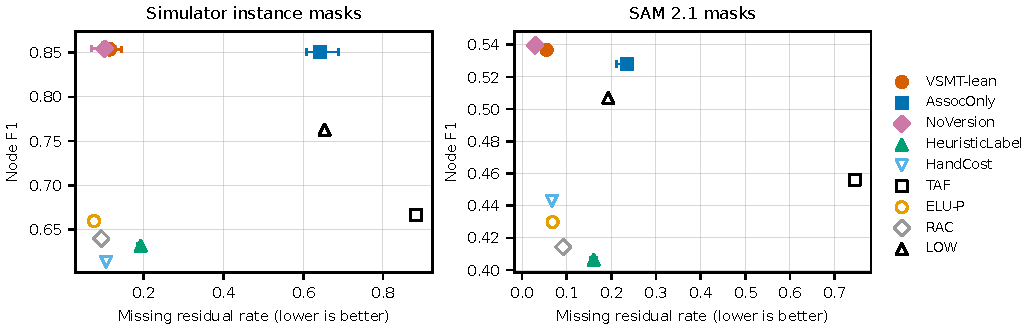
\includegraphics[width=0.9\linewidth]{figures/tradeoff}
\caption{Stale entities against node accuracy on test. Learned arms (filled) with the range over five seeds; rule-based arms and \arm{HandCost} (open) are deterministic. With instance masks no arm is best on both axes; with SAM~2.1 masks the deletion ablation \arm{NoVersion} is best on both axes but keeps almost no identities (identity continuity 0.014, Table~\ref{tab:main}).}
\label{fig:tradeoff}
\end{figure*}

No method dominates on every metric (Table~\ref{tab:main}, Fig.~\ref{fig:tradeoff}; intervals in Table~\ref{tab:rules}, Appendix~\ref{app:intervals}).
The originally registered gate against the strongest rule-based control is not met on either front end: with instance masks \arm{ELU-P} leaves fewer stale entities (0.075 vs.\ 0.115), while 92.4\% of the in-scope entities it retracts (96.7\% overall) belong to objects that are still in place and its node F1 is 0.660 (VSMT-lean 0.853); with SAM~2.1 VSMT-lean has the lower Missing residual rate (0.055 vs.\ 0.068), but the advantage is not established.
\arm{ELU-P} selected the end of its registered grid in three parameters on both front ends; a wider grid might lower its MRR further, and we did not widen it after the test.
VSMT-lean retracts one to two orders of magnitude less often than the retracting rule arms (with instance masks 272 judged retractions per run on the 66 houses of the false-retract list, a seed mean, against 9,492 for \arm{RAC} and 20,901 for \arm{ELU-P}).
Its in-scope false-retract rate (0.192 with instance masks, 0.564 with SAM~2.1; 0.221 and 0.668 overall) is far below that of the rule-based arms that retract and of the \arm{HandCost} and \arm{HeuristicLabel} ablations (0.80--0.96 in scope) and, with instance masks, above \arm{NoVersion}'s (0.163); with SAM~2.1 more than half of the in-scope entities it retracts belong to objects that remained in place.
Retracting a redundant part entity of an over-segmented object also counts as false, since identity is the majority object; the exports do not separate the two cases.
Identity continuity is higher than for every rule arm with instance masks (lower bounds $\geq +0.124$); with SAM~2.1 it is higher than \arm{ELU-P} and \arm{RAC}, not separated from \arm{TAF} and \arm{LOW}, and below \arm{HandCost}.
Retrieval is higher than for \arm{TAF} and \arm{LOW}, but its advantage over the retracting arms is not established (with SAM~2.1 it is below \arm{HandCost}).
Contamination AUC is lower than for every rule arm with instance masks, but with SAM~2.1 VSMT-lean, \arm{NoVersion} and \arm{AssocOnly} (0.462--0.466) are above \arm{TAF}, \arm{ELU-P}, \arm{RAC}, \arm{HandCost} and \arm{HeuristicLabel} (0.397--0.419) and below \arm{LOW} only (0.517); we did not investigate why, and this metric judges staleness by centroid distance only.
VSMT-lean's secondary node column (F1$_\mathrm{IoU}$: 0.490 with instance masks, 0.257 with SAM~2.1) uses Dyn-THOR's matching and overlap rule on different data and is not comparable with numbers in~\cite{dsg2026}.

\subsection{Where the errors are}
Every decision of every run falls into exactly one ledger class (Appendix~\ref{app:ledger}); VSMT-lean and \arm{AssocOnly} miss the correct candidate in recall about equally often in absolute terms (19,885 and 19,242 per run with instance masks).
With SAM~2.1 the share of ambiguous labels about doubles (12.7\% vs.\ 6.8\% for VSMT-lean), suggesting that part of the difficulty lies in the labels; about 10\% of its SAM~2.1 decisions are duplicate fragments.
Arms make different decisions (\arm{AssocOnly} only association decisions), so shares are not ranked across arms, and the ledger does not attribute the gate results to error classes.

\subsection{External check on 3RScan}
\label{sec:external}

\begin{table*}[t]
\centering
\caption{3RScan validation, instance masks rendered from the annotated meshes (proxy truth), every configuration frozen (no retraining or selection). Means over the scenes each metric's list keeps; last rows: advantage of VSMT-lean over \arm{AssocOnly} with the two-level 90\% interval ($^{\ast}$: seed-stability condition holds; this does not imply that the interval excludes zero). Descriptive; not part of the primary hypothesis.}
\label{tab:external}
\scriptsize
\setlength{\tabcolsep}{3pt}
% generated by paper/tools/make_tables.py from results/vsmt_lean_s3_07_statistics_aa94373.json; do not edit by hand

\begin{tabular}{lccccccccc}
\toprule
Arm & F1 & F1$_{\mathrm{IoU}}$ & MRR$\downarrow$ & FRR$\downarrow$ & FRR$_{\mathrm{in}}\!\downarrow$ & IdC & Retr. & Lat.$\downarrow$ & Cont.$\downarrow$ \\
\midrule
\textbf{VSMT-lean} & 0.582{\tiny$\pm$.008} & 0.162{\tiny$\pm$.001} & 0.111{\tiny$\pm$.021} & 0.412{\tiny$\pm$.031} & 0.369{\tiny$\pm$.030} & 0.438{\tiny$\pm$.046} & 0.425{\tiny$\pm$.025} & 24.0{\tiny$\pm$5.9} & 0.531{\tiny$\pm$.005} \\
AssocOnly & 0.543{\tiny$\pm$.018} & 0.161{\tiny$\pm$.002} & 0.137{\tiny$\pm$.039} & -- & -- & 0.338{\tiny$\pm$.089} & 0.351{\tiny$\pm$.086} & 25.4{\tiny$\pm$4.9} & 0.561{\tiny$\pm$.010} \\
NoVersion & 0.583{\tiny$\pm$.009} & 0.162{\tiny$\pm$.001} & 0.118{\tiny$\pm$.025} & 0.408{\tiny$\pm$.040} & 0.369{\tiny$\pm$.010} & 0.351{\tiny$\pm$.074} & 0.407{\tiny$\pm$.050} & 24.6{\tiny$\pm$6.5} & 0.530{\tiny$\pm$.006} \\
HeuristicLabel & 0.437{\tiny$\pm$.001} & 0.151{\tiny$\pm$.000} & 0.599{\tiny$\pm$.017} & 0.744{\tiny$\pm$.002} & 0.664{\tiny$\pm$.002} & 0.390{\tiny$\pm$.007} & 0.411{\tiny$\pm$.041} & 26.3{\tiny$\pm$2.6} & 0.398{\tiny$\pm$.001} \\
HandCost & 0.443 & 0.153 & 0.480 & 0.773 & 0.701 & 0.402 & 0.378 & 19.2 & 0.404 \\
TAF & 0.470 & 0.159 & 0.686 & -- & -- & 0.167 & 0.159 & 24.0 & 0.416 \\
ELU-P & 0.438 & 0.154 & 0.594 & 0.779 & 0.703 & 0.061 & 0.159 & 33.8 & 0.397 \\
RAC & 0.436 & 0.153 & 0.460 & 0.725 & 0.635 & 0.061 & 0.186 & 17.1 & 0.397 \\
LOW & 0.591 & 0.170 & 0.623 & -- & -- & 0.000 & 0.113 & 17.7 & 0.436 \\
\emph{Scenes kept} & 46 & 46 & 38 & 15 & 14 & 11 & 11 & 32 & 46 \\
\midrule
\emph{Adv.\ vs.\ AssocOnly} & +0.039$^{\ast}$ & +0.001 & +0.026 & -- & -- & +0.100$^{\ast}$ & +0.074 & +1.5 & +0.030$^{\ast}$ \\
\emph{\quad 90\% interval} & {\tiny[+0.022, +0.056]} & {\tiny[$-$0.003, +0.006]} & {\tiny[$-$0.031, +0.081]} &  &  & {\tiny[$-$0.004, +0.221]} & {\tiny[$-$0.044, +0.205]} & {\tiny[$-$7.4, +9.9]} & {\tiny[+0.021, +0.038]} \\
\bottomrule
\end{tabular}

\end{table*}

We paired reference scans and rescans of the 3RScan validation split~\cite{rio2019} into 108 usable episodes in 46 scenes; the window between scans has no frames, and poses and alignment come from offline reconstruction.
On these scenes, with instance masks rendered from the annotated meshes (proxy truth) and every configuration frozen, VSMT-lean has a higher node F1 than the association-only ablation ($+0.039$, 90\% interval $+0.022$ to $+0.056$) and leaves fewer stale entities, fewer false retractions and fewer lost identities than the rule-based arms; its advantages over the association-only ablation in Missing residual rate ($+0.026$, $-0.031$ to $+0.081$) and identity continuity ($+0.100$, $-0.004$ to $+0.221$; 11 scenes) are not established, and its contamination AUC is higher than that of every non-learned arm (Table~\ref{tab:external}).
Counter to ProcTHOR, \arm{LOW} has the highest node F1 (0.591; VSMT-lean $-0.009$, $-0.035$ to $+0.017$), \arm{AssocOnly}'s MRR is low (0.137 against 0.642 on ProcTHOR) and the rule arms' are high (0.46--0.69); we did not investigate why.
The SAM~2.1 column could not be computed with the frozen front end (3 of 110 episodes usable).
This check does not show that the primary result reproduces on real data, nor how a learned segmenter or a real robot would fare.

\textbf{Zero-training LLM operator.}
A frozen LLM choosing the same operations from the same sealed feature tables is reported in Appendix~\ref{app:llm}; it is not in the main table and no claim depends on it.

\section{Limitations}
\label{sec:limitations}

The primary hypothesis holds, for this training procedure, only with simulator instance masks, which reveal no identity but are close to perfect; with SAM~2.1 only the stale-entity reduction holds, and more than half of the in-scope entities VSMT-lean retracts belong to objects still in place.
Poses are the simulator's, changes happen only between containers, the test has 139 moved objects, and IdC scores only the first observation after a move; the 3RScan check uses proxy truth, no frames between scans and offline poses, and no real-robot experiment was run.
The rule-based arms are our re-implementations, several selections lie at the end of their grids, \arm{AssocOnly} has no parameter to select, and the two-level bound for five seeds was calibrated only by a null simulation.
The hypothesis was revised, and the fixed order and the identity-continuity definition were designed, after development and confirmation readings, though before validation and test; comparisons outside the fixed-order test are descriptive and partly computed after the test.

\section{Conclusion}
\label{sec:conclusion}

We tested whether a learned, versioned lifecycle vocabulary helps object-level memory under changes made outside the robot's view, holding the front end, recall, executor, training recipe and evaluation fixed and comparing against the same learned association without that vocabulary.
Under a protocol frozen before validation and test, with a single test read, the answer for this training procedure (five seeds) is yes for near-ideal instance masks on both stale entities and identity continuity, and yes for stale entities only with SAM~2.1 masks.
In a descriptive ablation, identity continuity depends on keeping the versions of retracted entities: deleting them leaves slightly fewer stale entities but loses the identities.
Against the rule-based adapters there is no single winner: with instance masks the persistence-filter adapter leaves fewer stale entities, while most of the in-scope entities it retracts belong to objects that are still in place.
The low absolute identity continuity, especially with a learned segmenter, is the main open problem; the released ledger, exports and index are meant to make that problem measurable.


\bibliographystyle{IEEEtran}
\bibliography{refs}

% No appendix: RA-L counts every page (6 + at most 2 paid pages, including figures, tables, references and appendices)
% and accepts only videos, data sets, code and documentation as supplementary material, so the main text is self-contained.

\end{document}
